\documentclass[a4paper]{report}
\usepackage[round]{natbib}


\usepackage{Rnews}
\usepackage{fancyvrb}
\usepackage{Sweave}

\DefineVerbatimEnvironment{Sinput}{Verbatim}{fontsize=\small,fontshape=sl}
\DefineVerbatimEnvironment{Soutput}{Verbatim}{fontsize=\small}
\DefineVerbatimEnvironment{Scode}{Verbatim}{fontsize=\small,fontshape=sl}


\bibliographystyle{abbrvnat}

\begin{document}
\begin{article}

\title{Analyzing an Electronic Limit Order Book}
\author{David Kane, Andrew Liu and Khanh Nguyen}

%%\VignetteIndexEntry{Using the orderbook package}
%%\VignetteDepends{orderbook}

\maketitle


\setkeys{Gin}{width=0.95\textwidth}

\section{Introduction}

The \pkg{orderbook} package provides facilities for exploring and
visualizing the data associated with an order book: the electronic
collection of the outstanding limit orders for a financial instrument,
e.g. a stock. A \dfn{limit order} is an order to buy or sell a given
quantity of stock at a specified limit price or better. The
\dfn{size} is the number of shares to be bought or sold.  An order
remains in the order book until fully executed, i.e. until its size is
zero as a result of trades. Partial executions occur as a result of
trades for less than the entire size of the order.

Consider a simple order book containing five limit orders: sell 150
shares of IBM at \$11.11, sell 150 shares of IBM at \$11.08, buy 100
shares of IBM at \$11.05, buy 200 shares of IBM at \$11.05, and buy
200 shares of IBM at \$11.01.

\begin{verbatim}
                 Price          Ask Size

                 $11.11         150
                 $11.08         100
     300         $11.05
     200         $11.01

Bid Size         Price
\end{verbatim}

\noindent Orders on the \dfn{bid} (\dfn{ask}) side represent orders to buy
(sell). The price levels are \$11.11, \$11.08, \$11.05, and
\$11.01. The \dfn{best bid} at \$11.05 (highest bid price) and the
\dfn{best ask} at \$11.08 (lowest ask price) make up the \dfn{inside
  market}. The \dfn{spread} (\$0.03) is the difference between the
best bid and best ask. The \dfn{midpoint} (\$11.065) is the average
of the best bid and best ask.

There are four types of messages that traders can submit to an order
book: \dfn{add}, \dfn{cancel}, \dfn{cancel/replace}, and
\dfn{market order}. A trader can \dfn{add} a limit order in to the
order book.  She can also \dfn{cancel} an order and remove it from
the order book. If a trader wants to reduce the size of her order, she
can issue a \dfn{cancel/replace}, which cancels the order, then
immediately replaces it with another order at the same price, but with
a lower size. Every limit order is assigned a unique ID so that cancel
and cancel/replace orders can identify the corresponding limit
order. A \dfn{market order} is an order to immediately buy or sell a
quantity of stock at the best available prices. A trade occurs when a
market order ``hits'' a limit order on the other side of the inside
market.

All orders have timestamps indicating the time at which they were
accepted into the order book. The timestamp determines the \dfn{time
  priority} of an order. Earlier orders are executed before later
orders. For example, suppose that the order to buy 100 shares at
\$11.05 was submitted before the order to buy 200 shares at
\$11.05. Now suppose a market order selling 200 shares is submitted to
the order book. The limit order for 100 shares will be executed
because it is at the front of the queue at the best bid. Then, 100
shares of the order with 200 total shares will be executed, since it
was second in the queue. 100 shares of the 200 share order remain in
the order book at \$11.05.

A market order for more shares than the size at the inside market will
execute at worse price levels until it is complete. For example, if a
market order to buy 200 shares is submitted to the order book, the
order at \$11.08 will be fully executed. Since there are no more
shares available at that price level, 100 shares at the \$11.11 price
level will be transacted to complete the market order. An order to
sell 50 shares at \$11.11 will remain in the order book. Executing
these two market orders (a sell of 200 shares and a buy of 200 shares)
on our hypothetical order book results in a new state for the order
book.

\begin{verbatim}
                 Price          Ask Size

                 $11.11         50
     100         $11.05
     200         $11.01

Bid Size         Price
\end{verbatim}

Note that cancel/replace orders can lower the size of an order, but
not increase it. Cancel/replace orders maintain the time priority of
the original order, so if size increases were allowed, traders with
orders at the highest time priority for a price level could
perpetually increase the size of their order, preventing others from
being able to transact stock using limit orders at that price
level. See \cite{johnson:barry} for more details on the order book.

\section{Example}

NVIDIA is a graphics processing unit and chipset developer with ticker
symbol NVDA. Consider the order book for NVDA at a leading electronic
exchange on June 8, 2010. We create the \texttt{orderbook} object by
specifying the location of our data file.

\begin{Schunk}
\begin{Sinput}
> library(orderbook)
> filename <- system.file("data",
+                         "sample.txt",
+                         package = "orderbook")
> ob <- orderbook(file = filename)
> ob <- read.orders(ob, 10000)
\end{Sinput}
\end{Schunk}
\begin{Schunk}
\begin{Sinput}
> ob
\end{Sinput}
\begin{Soutput}
An object of class orderbook (default)
--------------------------
Current orderbook time:    09:35:02 
Message Index:             10,000 
Bid Orders:                631 
Ask Orders:                1,856 
Total Orders:              2,487 
\end{Soutput}
\end{Schunk}

We read in the first 10,000 messages then \texttt{show} the object.
The current time is 9:35:02 AM. The message index indicates which row
in the data file the object has read through. The display also shows
that there are 631 bids and 1,856 asks outstanding, for a total of
2,487 orders. This indicates that many earlier orders have been
removed through either cancels or trades.

\begin{Schunk}
\begin{Sinput}
> summary(ob)
\end{Sinput}
\begin{Soutput}
Current time is 09:35:02 

Ask price levels:   540 
Bid price levels:   179 
Total price levels: 719 
-----------------------------
Ask orders:         1,856 
Bid orders:         631 
Total orders:       2,487 
-----------------------------
Spread:             0.02 

Mid point:          11.37 
-----------------------------
Inside market 
 
Best Bid:           11.36 
Size:               2,700 
 
Best Ask:           11.38 
Size:               400 
\end{Soutput}
\end{Schunk}

Using \texttt{summary} the total order information from \texttt{show}
is repeated. Additionally, we see that there are 540 ask and 179 bid
price levels, for a total of 719. This indicates that many orders
have been submitted at the same price level.  The spread is \$0.02,
and the midpoint is \$11.37. The inside market is composed of 2,700
shares offered at the best bid of \$11.36 and 400 shares offered at
the best ask of \$11.38.

\begin{Schunk}
\begin{Sinput}
> display(ob)
\end{Sinput}
\begin{Soutput}
Current time is 09:35:02 

		 Price 	 Ask Size
---------------------------------------------
		 11.42 	 900 
		 11.41 	 1,400 
		 11.40 	 1,205 
		 11.39 	 1,600 
		 11.38 	 400 
---------------------------------------------
  2,700 	 11.36 
  1,100 	 11.35 
  1,100 	 11.34 
  1,600 	 11.33 
    700 	 11.32 
---------------------------------------------
Bid Size 	 Price
\end{Soutput}
\end{Schunk}

\texttt{display} shows the inside market, along with the four next
best bid and ask price levels and the size at each price level.

\begin{figure}
\centering
\vspace*{.1in}
\begin{Schunk}
\begin{Sinput}
> plot(ob)
\end{Sinput}
\end{Schunk}
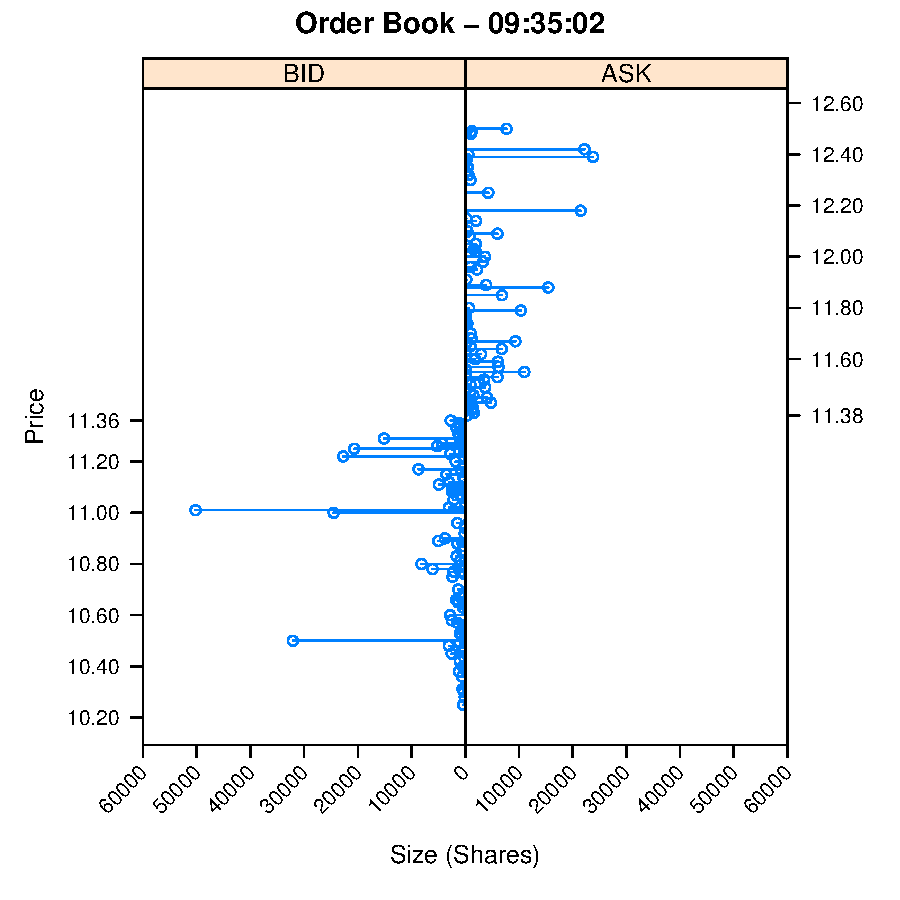
\includegraphics{orderbook-005}
\end{figure}

\texttt{plot} is a graphical representation of \texttt{display}. Price
levels are on the y-axis, and size is on the x-axis. The maximum and
minimum price levels displayed by default are 10\% above and below the
midpoint. Note the large number of shares at \$11.01. It is helpful to
know the number of orders which make up the large size at that price
level. Using the \texttt{"["} method we can view the order information
at particular price levels.

\begin{Schunk}
\begin{Sinput}
> ob["11.01"]
\end{Sinput}
\begin{Soutput}
  price  size type     time      id
1 11.01   109  BID 34220988 4403084
2 11.01 50000  BID 34220988 4403085
3 11.01   100  BID 34220988 4403086
\end{Soutput}
\end{Schunk}

There is an order for 50,000 shares at the \$11.01 price level that
accounts for almost all of the size.  We can view a plot of the number
of orders rather than the number of shares at each price level by
specifying \texttt{type = 'o'} when using \texttt{plot}. In the
previous plot the maximum and minimum price levels were 10\% off from
the midpoint, but for this plot we specify a range of only 3.3\%.

Note the large number of orders at \$11.00. The \texttt{"["} method
returns a \texttt{data.frame}, so we can use \texttt{nrow} to return
the number of orders at \$11.00.

\begin{Schunk}
\begin{Sinput}
> nrow(ob["11.00"])
\end{Sinput}
\begin{Soutput}
[1] 56
\end{Soutput}
\end{Schunk}

There are 56 orders at that price level, which confirms what
we see in the plot.

\begin{figure}
\centering
\vspace*{.1in}
\begin{Schunk}
\begin{Sinput}
> plot(ob, bounds = 0.033, type = 'o')
\end{Sinput}
\end{Schunk}
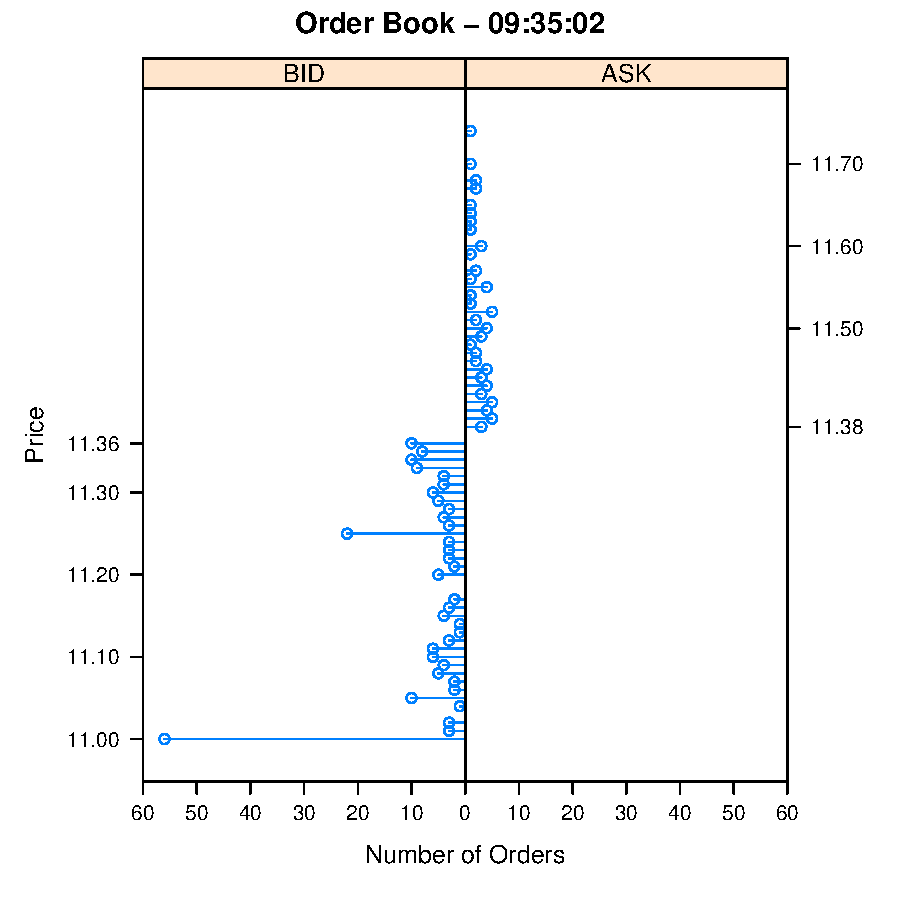
\includegraphics{orderbook-008}
\end{figure}

The type argument on plot allows for an ``sd'' option which shows
supply and demand curves for the order book. The demand (supply) curve
is downsloping (upsloping). This is because more people want to buy
(sell) a stock when the price decreases (increases). The ask (bid)
prices are normalized by the absolute value of the difference between
the highest (lowest) plotted ask (bid) price level and the the
midpoint. Following \cite{cao:orderbook}, the sizes are normalized by
the sum of the sizes across all plotted price levels for each
side.

\begin{figure}
  \centering
  \vspace*{.1in}
\begin{Schunk}
\begin{Sinput}
> plot(ob, bounds = 0.01, type = "sd")
\end{Sinput}
\end{Schunk}
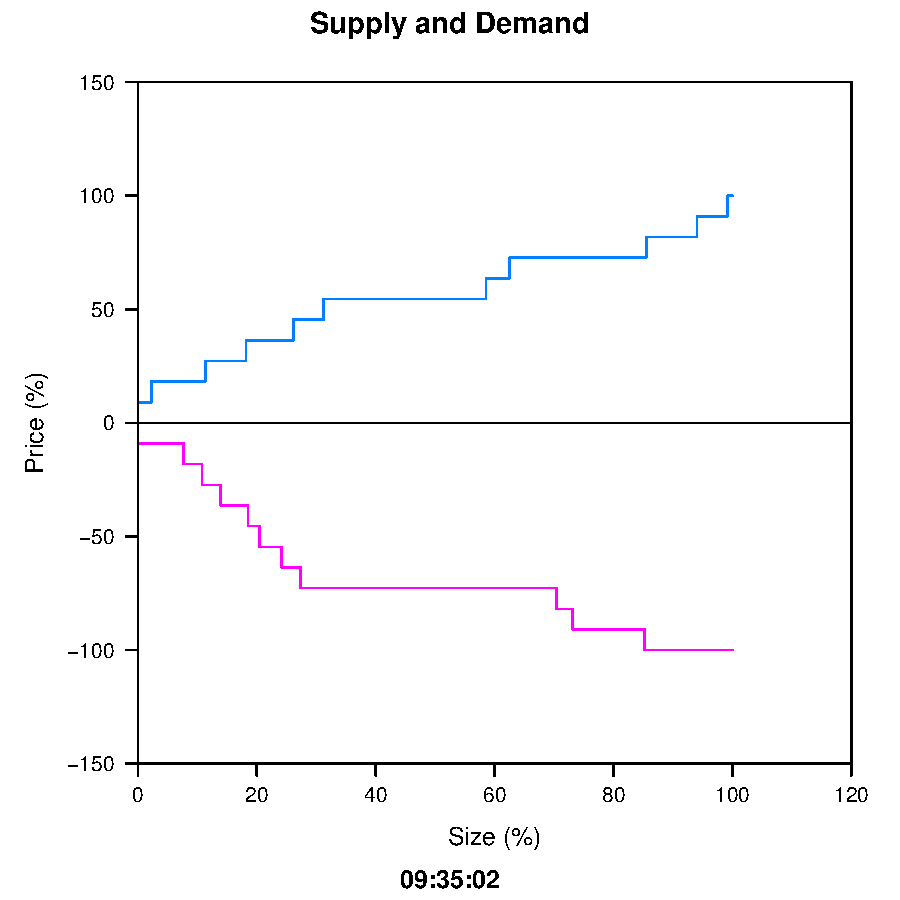
\includegraphics{orderbook-009}
\end{figure}

\pkg{orderbook} has methods for creating new \texttt{orderbook}
objects at specified clock times of interest. \texttt{read.time}
returns an \texttt{orderbook} object at the first message after the
specified time. For example, this returns the \texttt{orderbook}
object at 9:30:00.


\begin{Schunk}
\begin{Sinput}
> ob <- read.time(ob, "9:30:00")
\end{Sinput}
\end{Schunk}

\texttt{read.orders} is used to move forwards or backwards in the
order book by a specified number of messages. In this case, an
\texttt{orderbook} object at 50 messages before the current message is
returned.

\begin{Schunk}
\begin{Sinput}
> ob <- read.orders(ob, n = -50)
> ob
\end{Sinput}
\begin{Soutput}
An object of class orderbook (default)
--------------------------
Current orderbook time:    09:28:41 
Message Index:             292 
Bid Orders:                72 
Ask Orders:                81 
Total Orders:              153 
\end{Soutput}
\end{Schunk}

\section{Data}

Most brokers and exchanges have their own format for transmitting raw
order data to customers, so it would be unfeasible for us to write
scripts to automatically process all data formats. Consequently, raw
data for an \texttt{orderbook} object must be in the following form:

\begin{verbatim}
type,time,id,price,size,type,status
A,34226539,5920814,25.95,100,ASK,TRUE
A,34226788,5933949,25.91,100,BID,FALSE
R,34226900,5933949,50
C,34226904,5920814
T,34226904,755377,25.95,100,TRUE
\end{verbatim}

\noindent where A, R, T, and C mean Add, Replace, Trade, and Cancel,
respectively. The second column is the timestamp of the message in
milliseconds after midnight, and the third column is the order ID. For
a Replace the next column is the new size, while for Add and Trade a
column for price comes before the size column. Add messages also have
the type of order (BID/ASK) in the sixth column. The optional seventh
(sixth) column is \texttt{TRUE} if the order (trade) belongs to the
user, and \texttt{FALSE} otehrwise. This allows the user to create
plots that show the time priority of his own orders. If the column is
omitted, the first line of the data file should be \texttt{type, time,
  id, price, size, type} and not include \texttt{status}.

In this example a user order to sell 100 shares at \$25.95 is added to the
order book, followed by an order to buy 100 shares at \$25.91. The
 size of the order at \$25.91 is then replaced to 50 shares. Finally,
 the order at \$25.95 is cancelled, and a trade for 100 shares
 at \$25.95 occurs.

\section{Analyzing Trades}

A user can create plots that show the time priority of his own orders
if a \texttt{status} column is present in the data file.

\begin{Schunk}
\begin{Sinput}
> filename <- system.file("data",
+                         "tradersample.txt",
+                         package = "orderbook")
> ob <- orderbook(file = filename)
> ob <- read.time(ob, "9:30:05")
> ob <- next.trade(ob)
> ob
\end{Sinput}
\begin{Soutput}
An object of class orderbook (trader)
--------------------------
Current orderbook time:    09:30:05 
Message Index:             6,062 
Bid Orders:                164 
Ask Orders:                252 
Total Orders:              416 
\end{Soutput}
\end{Schunk}

Note that this \texttt{orderbook} object is of type trader.  The
\texttt{next.trade} function sets the state of the order book to when
the trade after the current time occurs. There is also a
\texttt{previous.trade} function with the same functionality moving
backwards

\begin{Schunk}
\begin{Sinput}
> view.trade(ob, tradenum = 584)
\end{Sinput}
\begin{Soutput}
       trade 584
row         6063
time    09:30:05
id        636783
price      25.94
size        1000
status     FALSE
\end{Soutput}
\begin{Sinput}
> mid.point(ob)
\end{Sinput}
\begin{Soutput}
 price 
25.935 
\end{Soutput}
\end{Schunk}

Since the trade price is higher than the midpoint price, we know that
the trade occurred as a result of an ask order getting hit. Note that
trade data is stored into the order book only after it has read
through the corresponding trade message.

\begin{Schunk}
\begin{Sinput}
> midpoint.return(ob, tradenum = 584, time = 10)
\end{Sinput}
\begin{Soutput}
          midpoint.return
10 second           0.065
\end{Soutput}
\end{Schunk}

The \dfn{midpoint return} is the difference in cents between the
execution price and the midpoint price after a specified period of
time. For example, the above calculates the ten second midpoint return
for the first trade. Since it was a sell order, the midpoint return
will be positive if the stock price decreases, and negative if the
stock price increases.

\begin{figure}
\centering
\vspace*{.1in}
\begin{Schunk}
\begin{Sinput}
> ob <- read.time(ob, "9:30:15")
> plot(ob, type = "t", bounds = 0.02)
\end{Sinput}
\end{Schunk}
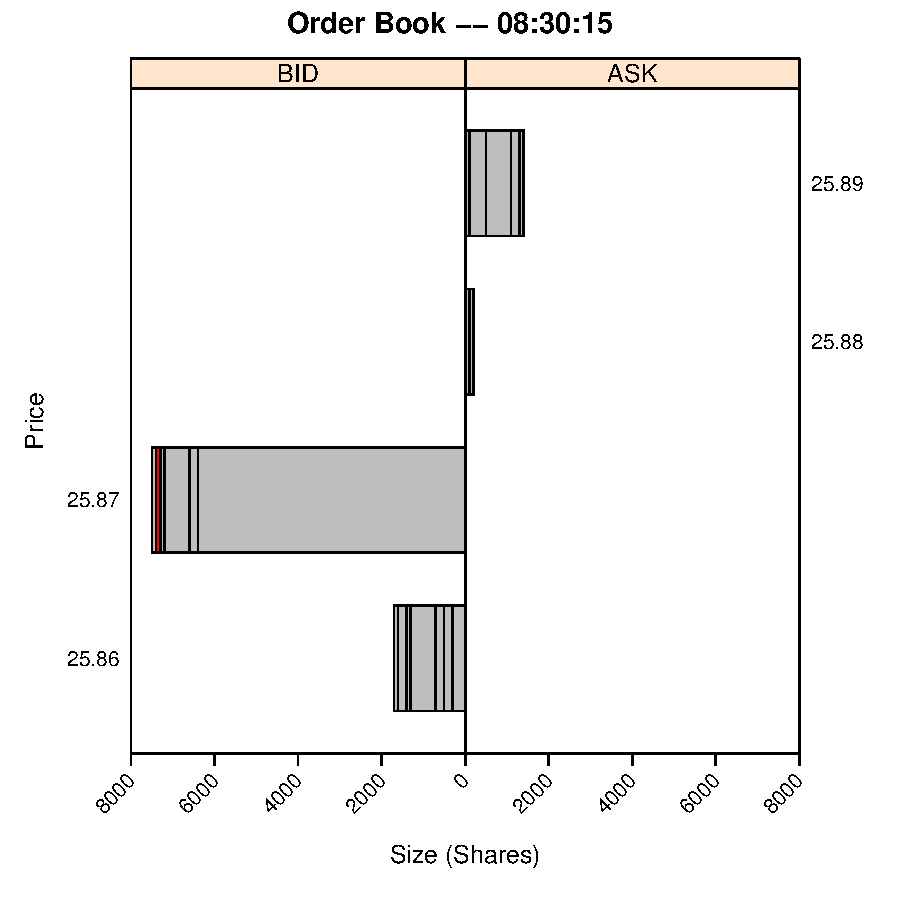
\includegraphics{orderbook-015}
\end{figure}

This plot shows two pennies above and below the best bid and best
ask. We see that the midpoint has dropped to 25.875, confirming the
midpoint return above. This graph shows two pennies above and below
the best bid and ask. Orders at these price levels are shown in time
priority, with the earliest submitted order being closest to the
middle y-axis. Note the red order--this is an order marked
\texttt{TRUE} by the user, indicating that it belonged to him.

\section{Simulation}

\pkg{orderbook} supports adding, replacing, and cancelling orders. Add
orders require the price, size, and type (ASK/BID) of the limit
order. Time and ID are optional, and will default to the maximum time
+ 1 and the maximum ID + 1. Replace messages require the new size and
ID. Cancel orders only require ID. In addition, market orders can be
issued to the order book. Market orders require size and side
(BUY/SELL).

\begin{Schunk}
\begin{Sinput}
> ob <- add.order(ob, 11.20, 300, "ASK")
> ob <- remove.order(ob, 1231883)
> ob <- replace.order(ob, 1231883, 150)
> ob <- market.order(ob, 200, "BUY")
\end{Sinput}
\end{Schunk}

Using these tools, the user can write functions to simulate the an
order book. In the following example, we consulted
\cite{gilles:daniel}. We simulate 1,000 messages.  The messages are
chosen based on the following probabilities: 50\% for a cancel
message, 20\% for a market order, and 30\% for a limit order. In the
event of a cancel message the order cancelled is randomly
chosen. Market order have a 50-50 chance for a buy or sell order. The
size of the market order always corresponds to the size of the
individual order at the best ask or bid with the highest time
priority. Limit orders have a 50-50 chance to be an ask or bid. There
is a 35\% chance for the price of a limit order to be within the
spread. If the price is outside of the spread, a price is chosen using
a power law distribution. Finally, the size follows a log-normal
distribution. A  plot of this example simulation is shown below.


\begin{Schunk}
\begin{Sinput}
> ob <- simulate(ob)
\end{Sinput}
\end{Schunk}
\begin{figure}
\centering
\vspace*{.1in}
\begin{Schunk}
\begin{Sinput}
> plot(ob)
\end{Sinput}
\end{Schunk}
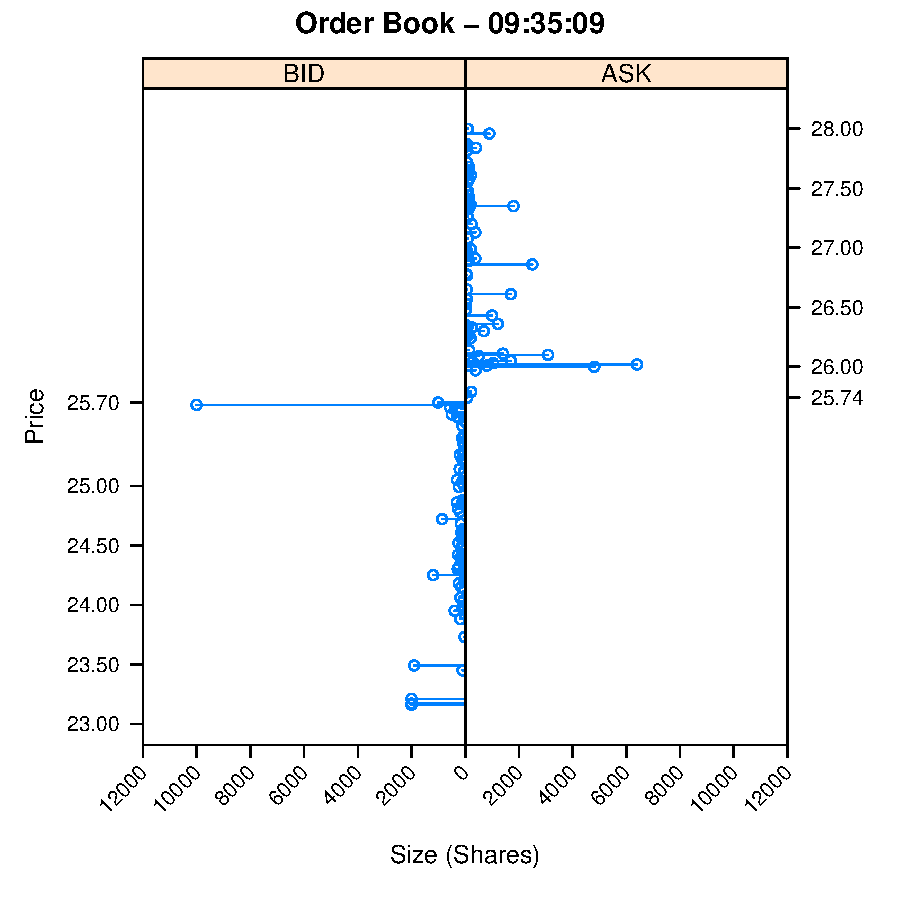
\includegraphics{orderbook-019}
\end{figure}

\section{Conclusion}

The \pkg{orderbook} package is part of a collection of packages (see
\cite{kane:backtest} and \cite{kane:portfolio}) for working with
financial market data. R provides all the necessary tools for
managing institutional sized portfolios.

\address{David Kane, Andrew Liu and Khanh Nguyen \\
  Kane Capital Management \\
  Cambridge, MA, USA\\
  \email{dave@kanecap.com}, \email{Andrew.T.Liu@williams.edu},
  and \email{knguyen@cs.umb.edu}
}

\bibliography{orderbook}
\end{article}
\end{document}
